\documentclass[a4paper]{scrreprt}

\usepackage[utf8]{inputenc}
\usepackage[T1]{fontenc}
\usepackage[acronym]{glossaries}
\usepackage{graphicx}
\usepackage{booktabs}
\usepackage{pdfpages}
\usepackage{hyperref}
\usepackage{listings}
\usepackage{tablefootnote}
\usepackage{verbatim}
\usepackage{multirow}
\usepackage{subcaption}
\usepackage{floatrow}
\usepackage{siunitx}
\usepackage{wasysym}
\usepackage{natbib}
\usepackage{physics}
\usepackage{hyperref}


\title{Development of an ultra-wide band indoor positioning system}
\author{Antoine Albertelli}
\titlehead{{\Large Ecole Polytechnique Fédérale de Lausanne}\\
    Laboratoire de Systèmes Robotique (LSRO)\\
    Supervisor: Daniel Burnier
}

\begin{document}

\newacronym{imu}{IMU}{Inertial Motion Unit}
\newacronym{dmp}{DMP}{Digital Motion Processor}
\newacronym{uwb}{UWB}{Ultra Wide Band}

\maketitle
\includepdf{abstract.pdf}
\tableofcontents

% TODO: Put each section in its own .tex
\chapter{Introduction}

\section{Requirements}

\section{State of the art}

\begin{enumerate}
    \item Sensor fusion using kalman for 9 axis IMUs is pretty common.
        Usually done using quaternions to represent rotations.
    \item Previous implementations of fusion with UWB focused on a applications of body positioning.
\end{enumerate}

\chapter{Hardware}

The board used in this project contains the following elements:

\begin{itemize}
    \item An Invensense MPU9250 \gls{imu}.
    \item A Decawave DW1000 \gls{uwb} transceiver.
    \item An STM32F411 microcontroller.
    \item USB and CAN interfaces.
\end{itemize}

\section{Inertial Motion Unit}

The MPU9250 is a 9 axis \gls{imu} made by Invensense\footnote{\url{https://www.invensense.com}}.
It was chosen because it combines an accelerometer, a gyroscope and a magnetometer in an easy to use package.
It is connected to the main microcontroller through an SPI bus.

An interesting feature of this device is the \gls{dmp}.
It is a low power co-processor that can be used for a variety of purpose, including orientation estimation, in which it directly outputs a quaternion.
Unfortunately, we found out that this feature is poorly documented by the manufacturer, making it impossible to use without reverse engineering.
Additionally, the \gls{dmp} cannot use the magnetometer data.
Therefore, we decided not to use it but to implement our own sensor fusion on top of raw sensor information.

\chapter{Positioning algorithm}

\section{Parametric vs non parametric filter}

Parametric filters are filter which take assumptions on the distribution of the state.
The most common assumption is that the distribution is Gaussian.
Non parametric filters, on the other hand, can represent any distribution, and most importantly multi modal ones.

If the problem can be solved using a parametric filter, it is better, as they are computationally less expensive.
Since we are running the code on a small device with little computing power, it is important to take this into account.

\section{First model}

The goal of this model was to create the simplest thing that could possibly work.
It does not account for most issues, but was enough to start work on a simulator for the system.

To simplify the model, the following hypotheses are made:
\begin{enumerate}
    \item The robot moves in the 2D plane, i.e. its pose is described by $\left( x, y, \theta \right)$.
    \item The \gls{imu}'s internal motion processor already outputs $\theta$ (but it drifts).
    \item The \gls{imu} outputs the acceleration vector in body frame $\mathbf{a}^b$.
    \item The inertial frame is aligned with the world frame, i.e. the robot starts with $\theta=0$.
\end{enumerate}

The state contains the position and speed, in world frame:
\begin{equation}
    \mathbf{x} = \begin{pmatrix}x & y & \theta & \dot{x} & \dot{y}\end{pmatrix}^T
\end{equation}

\subsection{Motion model}

The first step is to transform the acceleration from body frame to world frame.

\begin{equation}
    \mathbf{a}^w = R(\theta) \mathbf{a}^b
\end{equation}

The state update equation, using the acceleration as control input

\begin{eqnarray}
    \dv{t} \mathbf{x} &=&
    \begin{pmatrix}
        \dot{x} & 
        \dot{y} &
        0 & % TODO: Maybe take it from acceleration ?
        \mathbf{a}^w_x &
        \mathbf{a}^w_y
    \end{pmatrix}^T \nonumber
    \\&=&
    \begin{pmatrix}
        \dot{x} \\
        \dot{y} \\
        0 \\  % TODO: Maybe take it from acceleration ?
        \cos(\theta) \mathbf{a}^B_x - \sin(\theta) \mathbf{a}^B_y \\
        \sin(\theta) \mathbf{a}^B_x + \cos(\theta) \mathbf{a}^B_y \\
    \end{pmatrix}
\end{eqnarray}

We can turn it into a discrete state update equation using forward Euler:

\begin{equation}
    \mathbf{x}_{t+1} = \mathbf{x}_t + \Delta_t \dv{t} \mathbf{x}
\end{equation}


\subsection{Measurement model}
In this model we have two different measurement functions.
The first one is given by the \gls{dmp} and is directly the heading $\theta$:
\begin{equation}
    h_{DMP}(\mathbf{x}) = \theta
\end{equation}

The second type of measurement is the distance to the UWB anchors.
It is actually a family of functions; each beacon defines a measurement function.
This function is the distance to the position of the beacon, called $\mathbf{b}$.

\begin{equation}
    h_b(\mathbf{x}) = \sqrt{\left(\mathbf{x}_x - \mathbf{b}_x\right)^2 + \left(\mathbf{x}_y - \mathbf{b}_y\right)^2}
\end{equation}

\chapter{Implementation}

\section{UWB beacons protocol}

\subsection{Design principles}

\begin{enumerate}
    \item Stateless > stateful.
    \item Must maximize measurements per second -> minimize packets per measurements.
    \item The MAC layer should be used as much as possible to avoid waking up hosts.
    \item The same physical layer will also be used for data transmission.
    \item It must be noted that this protocol is possible only because the DW1000 can be programmed to \emph{send} messages at a given timestamp.
\end{enumerate}

\subsection{Time measurement}

\begin{figure}[h]
    \centering
    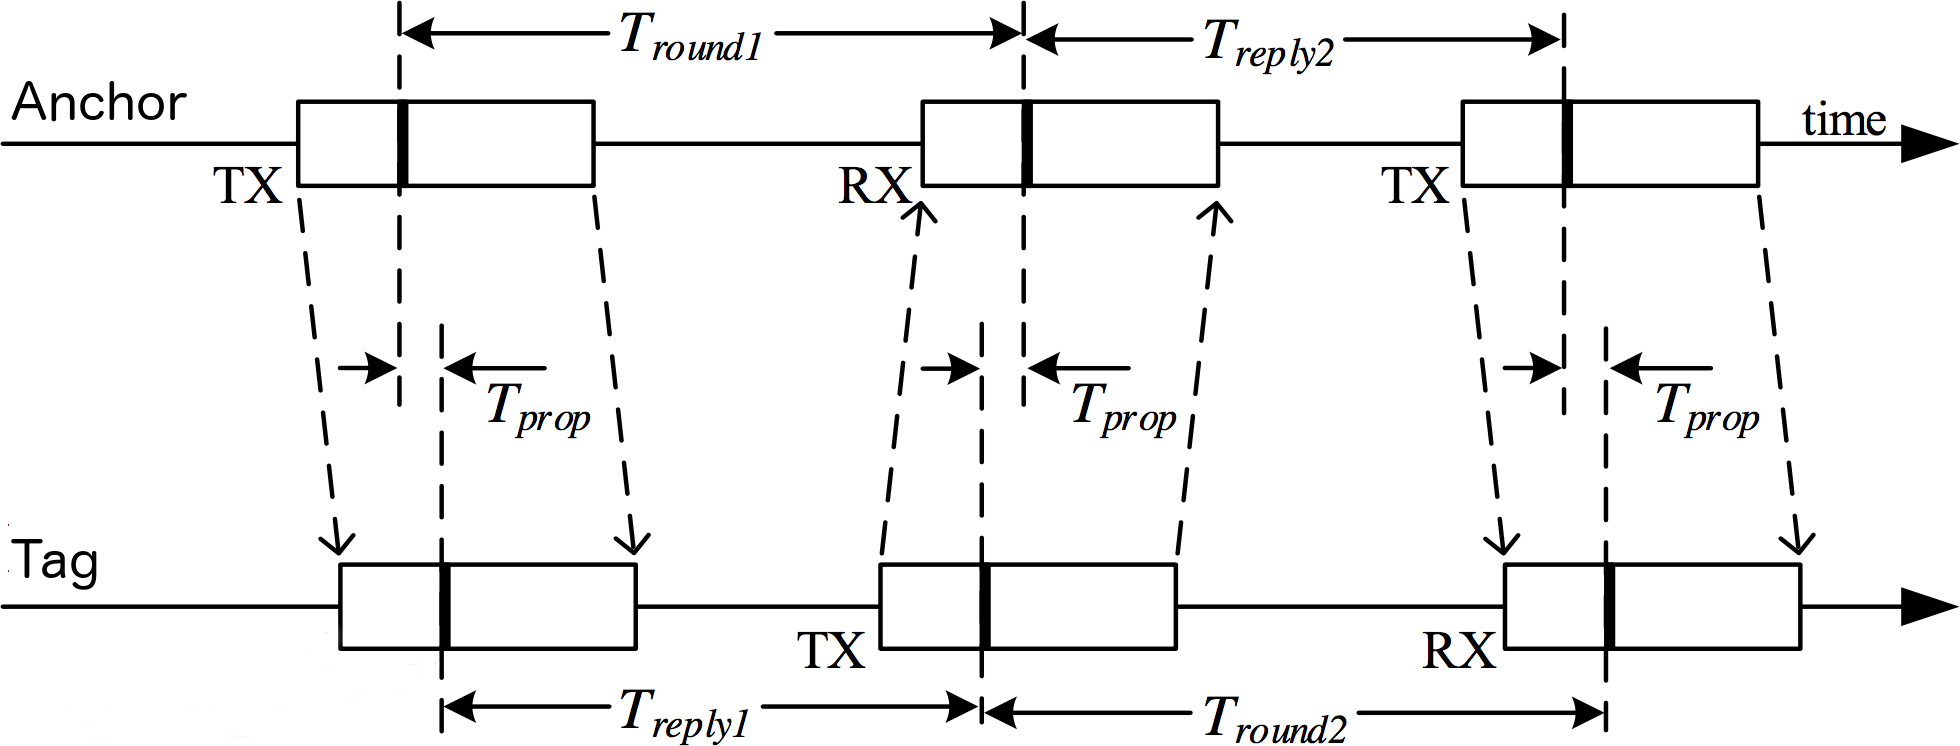
\includegraphics[width=0.8\textwidth]{figures/ranging_protocol.png}
    \label{fig:ranging_protocol}
    \caption[Ranging protocol]{Messages in a time measurement interaction. Source:~\cite{dw1000manual}}
\end{figure}

The time measurement protocol is composed of a sequence of 3 messages.
To initiate a measurement sequence, an anchor broadcasts a measurement advertisement message to the broadcast address (0xFFFF).
Tags may respond with a measurement reply message.
Finally, the anchor sends a measurement finalization message and the tag computes the ranging solution:

\begin{equation}
T_{prop} = \frac{T_{round,1} \cdot T_{round,2} - T_{reply,1} \cdot T_{reply,2}}{T_{round,1} + T_{round,2} + T_{reply,1} + T_{reply,2}}
\label{eqn:ranging}
\end{equation}

The timing information is then converted to a distance by multiplying by the speed of light ($c$).
\textbf{How do we convert time from DW1000 clocks to seconds?}

This 3-way ranging scheme works because transceivers can be programmed to send a frame at a given time.
Therefore, $T_{reply,2}$ can be included in the final message.

Some random implementations notes:

\begin{enumerate}
    \item Use 802.15.4 MAC to enable hardware filtering.
    \item Sequence number field will be hacked to store packet type in it instead.
    \item All numbers in payload are sent in network byte order (most significant byte first).
    \item All timestamps in messages are in DW1000 units and without a shared reference.
\end{enumerate}

\paragraph{Measurement advertisement}
A measurement advertisement message has a sequence number of 0.
It is sent by an anchor to the broadcast address (0xFFFF).
It only contains the TX timestamp as a 40 bit unsigned integer ($T_{tx,1}$).

\paragraph{Measurement reply}
A measurement reply message has a sequence number of 1.
It is sent by a tag and contains the timestamps of all events so far ($T_{tx,1}$, $T_{rx,1}$ and $T_{tx,2}$)

\paragraph{Measurement finalization}
Finally, the measurement finalization has a sequence number of 2.
It is sent by the anchor and contains the content of the previous message plus the new timestamps ($T_{rx,2}$, $T_{tx,3}$).

Once the tag received the last message, it can compute the ranging solution using Equation~\ref{eqn:ranging} with the following informations:
\begin{eqnarray*}
    T_{round,1} &=& T_{tx,1} - T_{rx,2} \\
    T_{reply,1} &=& T_{rx,1} - T_{tx,2} \\
    T_{round,2} &=& T_{tx,2} - T_{rx,3} \\
    T_{reply,2} &=& T_{rx,2} - T_{tx,3} 
\end{eqnarray*}


\subsection{Performance evaluation}

% TODO: Impact of antenna orientation
% TODO: Impact of preamble length

\appendix
\chapter{Hardware schematic}
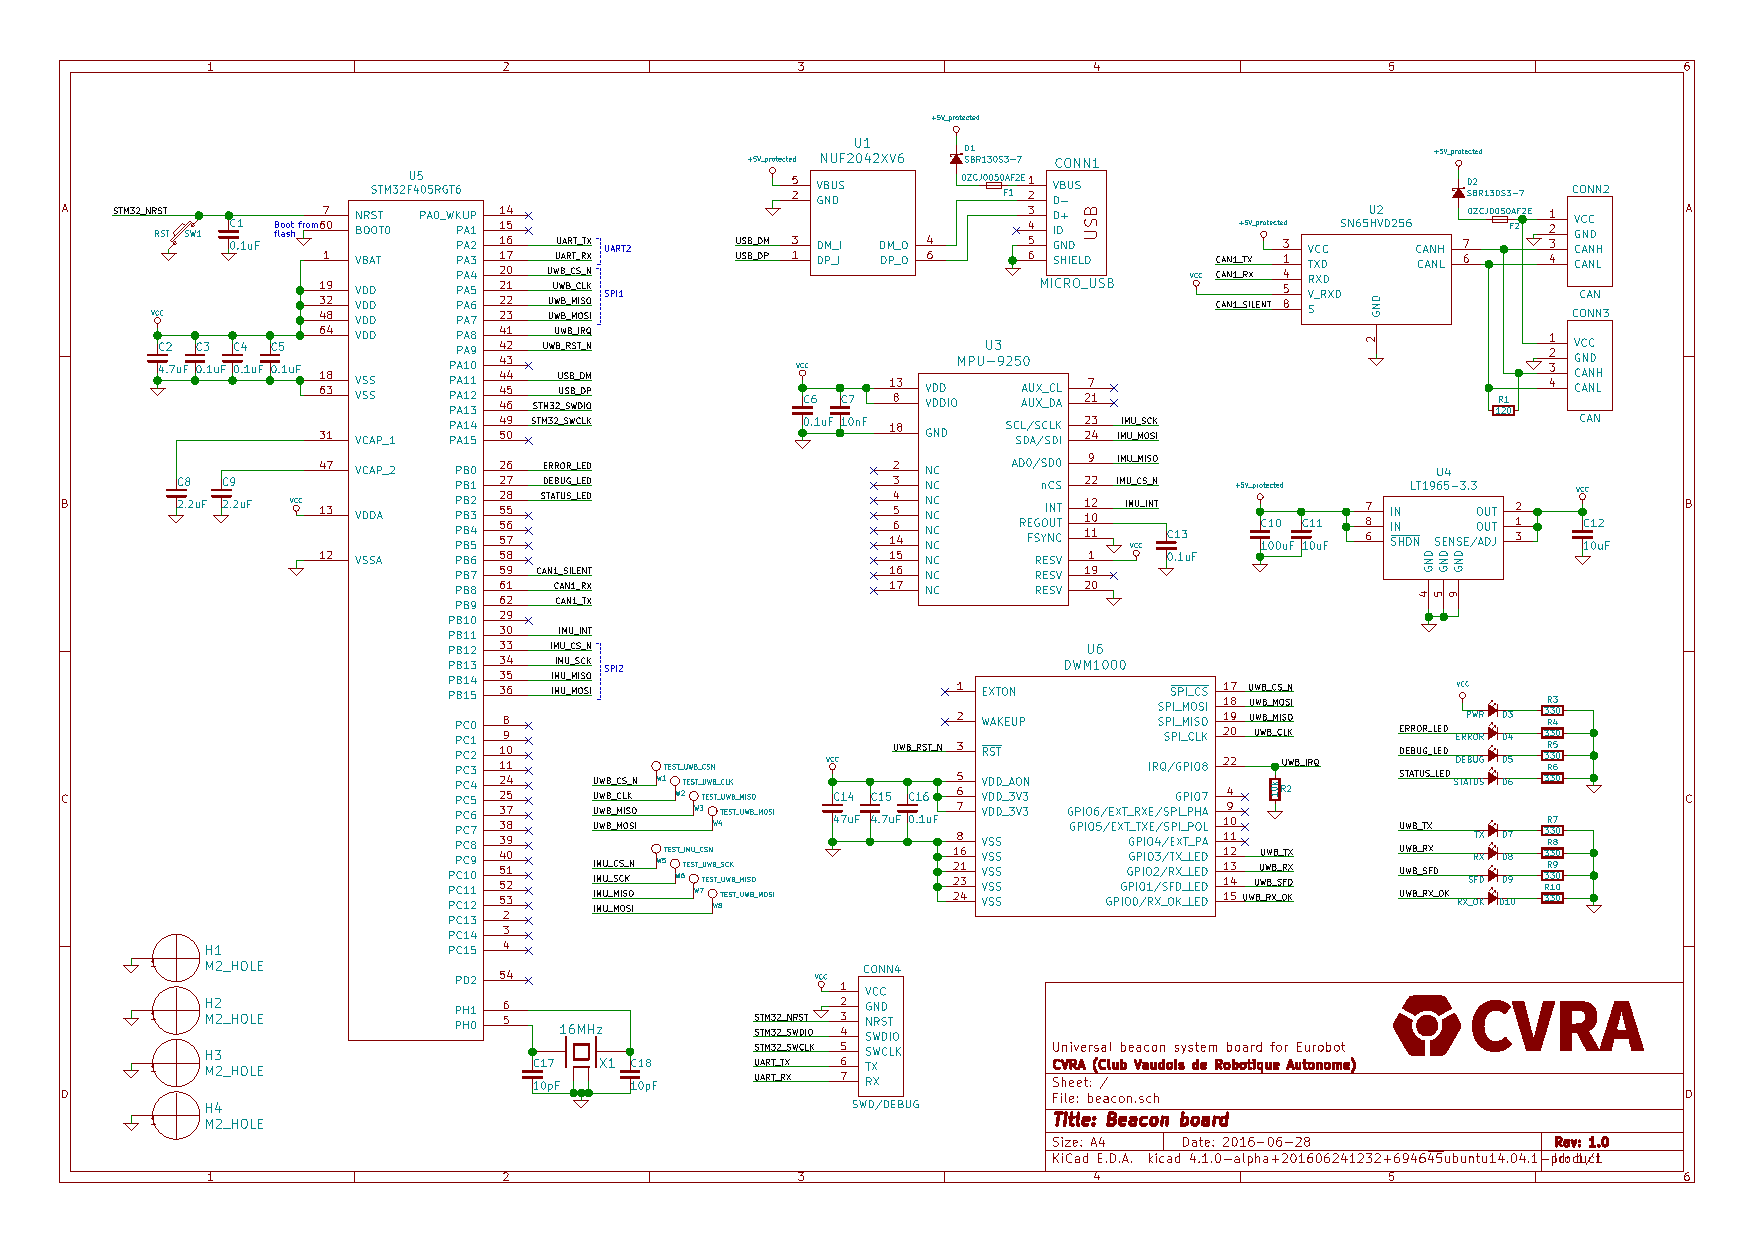
\includepdf[landscape=true]{figures/board_schematic.pdf}

\chapter{User manual}


\clearpage
\nocite{*} % tells bibtex to include everything
\bibliographystyle{chicago}
\bibliography{report}

\end{document}
